\documentclass{article}


\usepackage{arxiv}
\usepackage[utf8]{inputenc} % allow utf-8 input
\usepackage[T1]{fontenc}    % use 8-bit T1 fonts
\usepackage{hyperref}       % hyperlinks
\usepackage{url}            % simple URL typesetting
\usepackage{booktabs}       % professional-quality tables
\usepackage{amsfonts}       % blackboard math symbols
\usepackage{nicefrac}       % compact symbols for 1/2, etc.
\usepackage{microtype}      % microtypography
\usepackage{lipsum}
\usepackage{graphicx} 		% Used for Figures

\title{Deep Learning Project: GAN Artwork}


\author{
	Kevin Steele \\
	Department of Electrical and Computer Engineering \\
	University of Iowa\\
	\texttt{kevin-steele@uiowa.edu} \\
	%% examples of more authors
	\And
	Brain Fiegel \\
	Department of Industrial and Systems Engineering \\
	University of Iowa\\
	\texttt{brian-fiegel@uiowa.edu} \\
	\And
	Stjepan Fiolic \\
	Department of Electrical and Computer Engineering \\
	University of Iowa\\
	\texttt{stjepan-fiolic@uiowa.edu} \\
}

\begin{document}
	\maketitle
	
	\begin{abstract}
		The Iowa Neuroscience Institute has a desire for a landscape generation process by which DNA sequences are converted to landscape images. Our project is to train a Generative Adversarial Network (GAN) to accomplish this task. Specifically, we sought out the generative power of StackGAN as inspiration for image generation, using the general architecture to build a multi-stage network of increasing image fidelity. However, given that our data does not follow the same word-sentence input structure of the original paper, we were unable to use the architecture to the full extent. Our results are well enough given the difficulty of the task, but a simpler model might suit better for this possess. There is also room to grow with information extraction from the input sequence.

	\end{abstract}
	
	
	% keywords can be removed
	\keywords{Deep Learning \and GAN}
	
	
	\section{Introduction}
	\label{sec:intro}
	
	Generative Adversarial Networks (GANs) are an approach to generative modeling using deep learning methods. Generative models are an unsupervised machine learning task.  This task involves learning and discovering input data patterns in a way that the model can generate new output data that has a close relationship to the original input data. For example, if we were to feed the model with images of the human face, the model would generate a new human face that is not in the original dataset. This may be an example most people are familiar with, but models can also convert natural language text descriptions into images.  This type of model is called a Text-to-Image synthesis issue. We aim to achieve a similar goal by feeding a valid DNA sequence into our model and output a landscape image. 
	
	To understand GANs, the reader should first note that there are two sub-models of a GAN. The first is the generator model. The generator model takes a fixed-length random vector as input and generates a sample in that domain. A gaussian distribution is used to create a randomized vector. That vector then becomes the seed of the generative process. The training process will then produce latent (hidden) variables to input into the generator, the collection of which is referred to as a latent space. The second model of a GAN is the discriminator model. The discriminator model takes an example from the domain as input and predicts a binary class label.  This label is either authentic or generated. The authentic examples come from the training dataset, in our case images of landscapes. The generated examples come from the output of the generator model.  
	
	The best way to distinguish the two model types is to think about them as a tug of war. One model is trying to build a landscape image (generator) great enough to fool a human (discriminator) into thinking that it is a real landscape. The generator must make the landscapes as close to real landscapes while the human will point out flaws in the generated image and send it back.  
	
	There is a reward system in place between the generator fooling the discriminator and the discriminator.  This distinguishes the generated images from authentic images that come from the training set. If the generator is able to fool the discriminator, then the generator is rewarded by not having to rebuild its model.  In this case, the discriminator is punished by having to rebuild its model. Else-wise, if the discriminator correctly distinguishes a generated image, the generator is punished by having to rebuild its model.  The discriminator is rewarded by not having to rebuild its model. At convergence, the generator will have samples that are indistinguishable from the real data, or training set.  
	
	Conditional augmentation of a GAN is an extension where both the generator and discriminator take-in additional conditioning variables, in our case DNA.  The generator forms images based on the additional conditioning variables and the discriminator verifies. First question should be how to convert a DNA element to a string that represents a feature in a landscape image. We plan on using an encoder to map DNA codons.\footnote{sequence of three DNA nucleotides that corresponds with a specific amino acid or stop signal during protein synthesis.}  
	
	Given our particular object of Text-to-Image synthesis, we will require a specialized GAN architecture. A few architectures have been proposed in this realm, particularly StackGAN \cite{zhang2017stackgan} for text-to-image and CycleGAN \cite{CycleGAN2017} for unpaired image mapping. This process can be used for text-to-image as well \cite{BERT2020}, which involves using two generators, one mapping text to the generated image, then another doing the reverse with an image mapping to a generated text. A more recent attempt at this is MirrorGAN \cite{qiao2019mirrorgan}, which uses a stacked generator architecture to generate an image and an auto-encoder to regenerate semantically similar text. In examining the architectures, we decided to work with StackGAN. This architecture has two stages: stage-I GAN and stage-II GAN. Stage-I GAN does a rough estimation sketch of the text input provided. For a mountain landscape this would be the equivalent of having mountains distinguishable from sky but not being able to distinguish individual trees or different mountain faces. Stage-II uses the same text input that stage-I has and the low-resolution output image of stage-I as an input. This stage is where the details are included, like being able to distinguish mountain faces and trees.   
	
	Real world applications that we discussed include a provided digital image of a landscape generated based on the participant’s DNA. Although this might be a neat souvenir for the participant, some privacy concerns arise with participant DNA structure being transmitted over an unsecured connection. Also, the image would be a random conglomeration of DNA, but a clever enough person might be able to reconstruct participant data with the correct tools. 
	
	
	\section{Problem Definition}
	\label{sec:problemdef}
	Our goal is to convert a valid DNA input sequence into a landscape image using a Generative Adversarial Network (GAN). Examples of these can be seen in the Data section \ref{sec:data}. This is a Text-to-Image synthesis issue, with the generator taking valid DNA codons (TCAG) as input and creating landscape 224 by 224 by 3 (RBG) images as output. Image values range within [0,255] across the 3 color channels. Similar to a more general Text-to-Image GAN, which would take text descriptions to generate images, the DNA codon sequence will be a translated language by which we generate landscapes. Valid DNA codons follow the standard generic code table with valid inputs of T, C, A, and G in groups of 3. Each sequence must also start with a start codon and end with an end codon. Noted in the original table, there are 25 different amino acids that these codons correspond to. While it is not currently our goal, this fact could be used similarly to an alphabet, and thusly a sentence or description of the image.  

	Looking more comprehensively at the GAN, the generator takes as input valid codon, considered the latent space of the system, and outputs the image we desire. The discriminator would take as input an image, either directly from the dataset or from the generator, and return the probability that the image is real (direct input) or fake (generated input). It is obvious that, generally, DNA does not map to images in the real world. For our purposes, we currently create input to the generator, the latent variables, by converting the DNA sequence to a normalized average value between [0, 1]. Specifically, each character is represented by a number between 0 to 3 (ACGT respectively). These numbers are averaged by taking the sum of them and dividing by the length of the sequence and the length of a codon (3). This average is what we record, and thus we convert the variable length string into a single floating-point feature. This is done to create 128 latent variables, thus creating a 128-dimension latent space. Finally, the values are normalized to [0,1], finishing our noise generation. We played around with using text embeddings using k-mer counting and Sequence Graph Transformation, but ended up leaving this out as it would not conform to the latent space defined. It is an area with room for exploration, however. As for the landscape images, all images vary in resolution, many of which are far too large to train on, and thus must be down-sampled into their 224 by 224 format. This is handled by keras preprocessing when loading the dataset into training and testing sets. 

	
	\section{Data}
	\label{sec:data}
	The datasets used within this project are a Landscape dataset obtained from Kaggle and a DNA dataset obtained from Joint Research Center. They can be found at their respective pages:
	\begin{center}
		\url{https://www.kaggle.com/arnaud58/landscape-pictures} \\
		\url{https://data.jrc.ec.europa.eu/dataset/2abb5c2b-3ab6-4ce4-b103-cb1c5fc7349e}
	\end{center}

	\subsection{Landscape Dataset}
	The landscape dataset contains a variety of non-descriptive landscape images. There are no classifications or metadata for any image. All images start as JPEG images of varying sizes, but are pre-processed to be 224 by 224, as can be seen in Figure \ref{fig:landscapes}. The images used were scraped from Flickr images
	
	\begin{figure}[h]
		\centering
		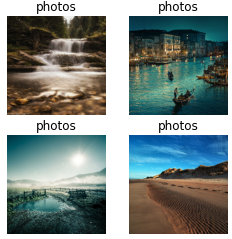
\includegraphics[scale=1]{images/landscapes}
		\caption{Pre-processed images}
		\label{fig:landscapes}
	\end{figure}

	
	\subsection{DNA Dataset}
	The DNA dataset contains various sequences of DNA codons. Collected by the Joint Research Center by sequencing genetically modified strains of bacillus subtilis used for production of vitamin B2 in feed additive. \\
	Data is formatted in a {\em .fastq} file with the structure found in Table \ref{tab:dna}.
	
	\begin{table}
		\caption{DNA Formatting}
		\centering
		\begin{tabular}{llllll}
			\toprule
			ID     & Name     & Description & Number of Features & Per letter annotation for: & Sequence \\
			\bottomrule
		\end{tabular}
		\label{tab:dna}
	\end{table}
	
	\section{Method}
	Here we will discuss the methodology of employed on the project. All code was developed to be run on Google Colab using Jupyter Notebook formatting for Python. Code can be found at \url{https://github.com/KaiwenS7/DeepLearningProject}.

	\subsection{Relevant Equations}

	\subsection{Implementation}
	We originally followed the StackGAN model as closely as was capable, implementing the neural networks of the stage 1 GAN and the stage 2 GAN without the conditional augmentation. In the original paper, conditional augmentation was used for word segmentation and sentence feature extraction, which is then fed into both stages. We do no such thing with DNA sequences. Both stages use an Adam optimizer with a Learning Rate of 0.0002 and a Beta of 0.5 for both the discriminator and the generator. We have also implemented a learning rate decay of 0.5 every 50 epochs.

	In preparation for discussion of each stage, we will first define the blocks used to simplify explanation of the models. There are 2 repeating blocks used in building the GANs, the Up Sample block and Down Sample block. The Up Sample block involves an up sampling layer followed by a convolutional layer with a ReLU activation. The Down Sample block is a convolutional layer of at least stride 2, followed by a ReLU activation and a Dropout layer. Also as a note, all LeakyReLU activations use an alpha of 0.2, and all Dropout layers use a 0.2 dropout rate.

	The stage 1 generator takes an input with the latent space size of 128. This is fed into a dense layer and reshaped with the values (4, 4, 1024). This is fed through a series of 4 Up Sample blocks, each reducing the filter size by half. Finally we use a convolution layer with 3 filters and a tanh activation to obtain a 64x64x3 image. The discriminator follows a convolutional layer of 64 filters and a kernel of 4 using a LeakyReLU activation. Following this is 4 Down Sample blocks, each doubling the number of filters, and finally the discriminator ends with a dense layer of output size 1, the probability that the input sample is real.

	The stage 2 generator follows the output of the stage 1 generator, taking the 64x64x3 image as input. Since we desire a 224x224x3 output, the input image must be resized to 56x56x3 using lanczos resampling \url{https://en.wikipedia.org/wiki/Lanczos_resampling}. This is fed through 2 Up Sample block of kernel 4 with filter sizes of 112 and 224 respectively, and the generator finishes with a convolutional layer of 3 filters  and a tanh activation output. This provides a 224x224x3 image. The discriminator opens with convolutional layer of filter size 224, kernel 4, and stride 2, followed by a LeakyReLU layer. This is then fed through 3 Down Sample blocks of kernel 4 and filters 56, 112, and 224 respectively. Finally, a dense layer of output size 1 generates the discriminator’s prediction.

	\subsection{Training}

	\section{Results and Discussion}
	

	\subsection{Evaluation}	


	\section{Conclusion}

	    A short summary of the work. Keep it brief and concise, and straight to the point.


	\bibliographystyle{unsrt}  
	%\bibliography{references}  %%% Remove comment to use the external .bib file (using bibtex).
	%%% and comment out the ``thebibliography'' section.
	
	
	%%% Comment out this section when you \bibliography{references} is enabled.
	\begin{thebibliography}{1}
		\bibitem{zhang2017stackgan}
		Han Zhang, Tao Xu, Hongsheng Li, Shaoting Zhang, Xiaogang Wang, Xiaolei Huang, and 
		Dimitris Metaxas.
		\newblock StackGAN: Text to Photo-realistic Image Synthesis with Stacked 
		Generative Adversarial Networks.
		\newblock {\em arXiv preprint arXiv:1612.03242}, 2017.
		

		\bibitem{CycleGAN2017}
		Zhu, Jun-Yan and Park, Taesung and Isola, Phillip and Efros, Alexei A.
		\newblock Unpaired Image-to-Image Translation using Cycle-Consistent Adversarial Networks.
		\newblock In IEEE International Conference on Computer Vision (ICCV), 2017.

		\bibitem{BERT2020}
		Trevor Tsue and Samir Sen and Jason Li
		\newblock Cycle Text-To-Image GAN with BERT
		\newblock {\em arXiv preprint arXiv:2003.12137}, 2020
		
		\bibitem{qiao2019mirrorgan}
		Tingting Qiao and Jing Zhang and Duanqing Xu and Dacheng Tao.
		\newblock MirrorGAN: Learning Text-to-image Generation by Redescription
		\newblock {\em arXiv preprint arXiv:1903.05854}, 2019.
		
	\end{thebibliography}
	
	
\end{document}